%%%
%%%
\chapter{Discrete probability}
%%%
%%%
We will follow the books~\cite{Newstead,DeGroot2012} in this chapter.
Some examples are just copied directly from these books., just as we distinguished the three coins in Example 1.6.3.

We now get to the final chapter of the course.
Probability is perhaps one of the most important concepts in human history.
Since the very ancient time, humans entertain themselves with probability by the
game of chance: gambling... 
This game is almost universal: as far as I can tell, every culture has a version
of gambling that ruins people's lives.
It is very interesting how this game is a universal phenomenon.

At its heart, probability is a little bit paradoxical: it tells us how to predict
randomness! How can one predict anything if everything is random?!
The main point is that probability does not tell you what is going to happen
to one particular sequence of events.
However, it will tell you how likely a sequence of events will happen
with some ``confidence''.
When one uses the language of probability, one needs to be careful not to treat
it as an absolute way to predict something but one needs to allow the possibility 
that the sequence of events under consideration may not happen.


\section{The basics}

In daily language, we talk about the probability of some event to happen 
to mean the following
\begin{equation*}
    \text{Probability of an event happening  }
    = \frac{\text{Number of times the event appear}}{\text{Total number of  outcomes}} \,.
\end{equation*}
Most of the time, we unconsciously think that all the events are equally likely such as the probability for a coin to be head or tail or the probability for a die to be $1,2,\dots, 6$.
This is because we \emph{assume} that there is no reason for the head to appear more often than the tail or $1$ to appear more often than $6$.

\begin{example}
    In daily life, we assume
   \begin{itemize}
       \item The probability for a fair coin to be head is $1/2$.
       \item The probability for a fair die to be 4 is $1/6$.
   \end{itemize} 
\end{example}

However, this assumptioin is not entirely well thought out as there are ways 
to make a coin land on its head more often than its tail.
The coin manufacturer could play with the physics to do it!




\begin{definition}
    Let $A$ be a set.
    The \emph{power set} of $A$, denoted by $\cP(A)$, 
is the set of all subsets of the set $A$. 
\end{definition}

\begin{example}
            $\cP(\set{1,2}) = \set{ \emptyset, \set{1}, \set{2}, \set{1,2}} $.
\end{example}



\begin{definition}
    A \emph{finite discrete probability space} is a pair $(\Omega, \P)$
    where $\Omega$ is a countable set
    and $\P:\cP(\Omega) \to [0,1]$ is a function such that
    \begin{enumerate}
        \item $\P(\Omega) = 1$,
        \item $\P(\bigcup_{i=1}^\infty A_i) = \P(A_1) + \P(A_2) + \dots$ when $A_i\cap A_j = \emptyset$ and $i\not = j$.
    \end{enumerate}
    The set $\Omega$ is called the \emph{sample space}, 
    an element $\omega \in \Omega$ is called an \emph{outcome}, 
    a subset $A \subseteq \Omega$ is called an \emph{event},
    Given $A$, $\P(A)$ is called the \emph{probability of $A$}.
\end{definition}
One can think of the sample space as the set of all possible outcomes. 
An observation based on the above definition is that
a sample space is also an event.

\begin{example}
   Let us model a coin toss.

   The outcomes of the toss are head or tail.
   So, we can take $\Omega = \set{H,T}$.

   The events correspond to the subsets of $\set{H,T}$:
   \begin{enumerate}
       \item $\P(\set{H}) = 1/2 = \P(\set{T})$,
       \item $\P(\emptyset) = 0$,
       \item $\P(\set{H,T}) = 1$.
   \end{enumerate}
\end{example}

\begin{example}
A slightly more interesting thing to talk about is modeling two coin tosses.
In this case, $\Omega = \set{HH, HT, TT,TH}$.
The first letter represents the outcome of the first toss and the second letter the outcome of the second toss.
Here's a few probabilities:
\begin{enumerate}
    \item $\P(\set{HT}) = \P(\set{HH}) = \P(\set{TT})= \P(\set{TT}) = 1/4$
    \item $\P(\set{H}) = \P(\set{HT, HH})  = 1/2$.
\end{enumerate}
\end{example}

\begin{exercise}
    Assume you have a fair coin. Write down the probability space  for three coin tosses.
\end{exercise}

\begin{example}
    Assume you have a fair die. Write down the probability space for one die toss.
    What is the probability for the die to be odd?

    A good way to visualize this is to draw a pie, color the parts that you're looking at and take the area of the colored part and divide it by the total pie.

    \begin{figure}[htpb]
        \centering
        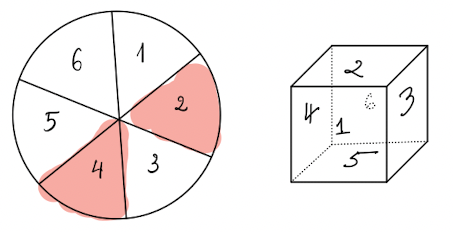
\includegraphics[width=0.8\linewidth]{Figures/pie}
        \caption{The ratio of the color part divided by the total number of equally divided parts gives the probability of the event
        that either the die turns out to be either 2 or 4.}%
        \label{fig:Pie}
    \end{figure}
\end{example}


\begin{proposition}[Some properties of probability]
   The followings are true.
   \begin{enumerate}
       \item $\P(A^C) = 1 - \P(A)$,
       \item $\P(\emptyset) = 0$,
       \item If $A\subseteq B$, then $\P(A) \leq \P(B)$,
       \item $\P(B \cap A^C) = \P(B) - \P(A\cap B)$,
       \item Inclusion-Exclusion principle:
           \begin{equation*}
            \P(A\cup B) = \P(A) + \P(B) - \P(A\cap B) \,.
           \end{equation*}
   \end{enumerate}
\end{proposition}

\begin{proof}
    Let's go through the list.
    \begin{enumerate}
        \item We know that $\Omega = A \cup A^C$ and that $\P(\Omega) = 1$.
            Thus,
            \begin{equation*}
                1 = \P(\Omega) = \P(A) + \P(A^C)\,.
            \end{equation*}
           Rearrange this, we have
           \begin{equation*}
              \P(A^C) = 1 - \P(A) \,. 
           \end{equation*}

       \item $\emptyset = \Omega^C$. Applying (1), we get
           \begin{equation*}
               \P(\emptyset) = 1 - \P(\Omega) = 1-1 = 0 \,.
           \end{equation*}

       \item $B = (B\setminus A) \cup A $. Thus,
           \begin{equation*}
               \P(B) = \P(B \setminus A) + \P(A) \geq \P(A)\,.
           \end{equation*}
           
       \item This follows by the following equation.
           \begin{equation*}
               \P(B) =  \P(B \cap A^C) + \P(B\cap A)\,.
           \end{equation*}
           Rearranging this, we get
           \begin{equation*}
               \P(B\cap A^C) = \P(B) - \P(A\cap B)\,.
           \end{equation*}

       \item We have that 
           \begin{equation*}
               A\cup B = A \cup (B \cap A^C)\,.
           \end{equation*}
           Therefore, using (4),
           \begin{equation*}
            \P(A \cup B) = \P(A) + \P(B \cap A^C) = \P(A) + \P(B) - \P(A \cup B)\,.
           \end{equation*}
    \end{enumerate}
\end{proof}

\begin{example}
   A patient arrives at a doctor’s office with a sore throat and low- grade fever. After an exam, the doctor decides that the patient has either a bacterial infection or a viral infection or both. The doctor decides that there is a probability of 0.7 that the patient has a bacterial infection and a probability of 0.4 that the person has a viral infection. What is the probability that the patient has both infections? 
\end{example}

\begin{example}
    Inherited traits in humans are determined by material in specific locations
on chromosomes. Each normal human receives 23 chromosomes from each parent,
and these chromosomes are naturally paired, with one chromosome in each pair coming from each parent. For the purposes of this text, it is safe to think of a gene as a portion of each chromosome in a pair. The genes, either one at a time or in combination, determine the inherited traits, such as blood type and hair color. The material in the two locations that make up a gene on the pair of chromosomes comes in forms called alleles. Each distinct combination of alleles (one on each chromosome) is called a genotype.

Consider a gene with only two different alleles A and a. Suppose that both parents have genotype Aa, that is, each parent has allele A on one chromosome and allele a on the other. (We do not distinguish the same alleles in a different order as a different genotype. For example, aA would be the same genotype as Aa. But it can be convenient to distinguish the two chromosomes during intermediate steps in probability calculations.) What are the possible genotypes of an offspring of these two parents? If all possible results of the parents contributing pairs of alleles are equally likely, what are the probabilities of the different genotypes? 
\end{example}


\section{Probability from counting }
Let us learn how to come up with probability law for 
some``simple'' situations, where the number of outcomes is finite. 
We call this finite probability (as opposed to countably inifinite probability).
We will assume that every outcome is equally likely to another
and, hence, in order to determine the probability of an event, one needs to be
able to count accurately.
The general principle is
\begin{equation}
    \label{eq:gen-principle}
    \text{Probability of an event happening  }
    = \frac{\text{Number of ways it can appear}}{\text{Total number of  outcomes}} \,.
\end{equation}

\begin{example}
    Let $A_3$ be the graph in homework 8.
    Suppose we have 4 colors: red, blue, yellow, green.
    Assume that each coloring is equally likely. Write down 
    the probability space for the chance for a particular way of coloring is chosen.
\end{example}

\begin{example}
    Let $K_3$ be the complete graph with 3 vertices.
    Suppose we have 4 colors: red, blue, yellow, green.
    Assume that each coloring is equally likely. Write down 
    the probability space for the chance for a particular way of coloring is chosen.
\end{example}
Thus, it is important to learn how to count.

\subsection{Counting}
In order to apply the general principle~\ref{eq:gen-principle}, we need to know
the total number of outcomes.
One could list them all out. However, when the number of outcomes gets large,
this is very inefficient and often leads to errors.
It is nice to have a way (formula) to find the total number of outcomes efficiently.
This section will discuss several ways, which we can use to do just that.


\begin{example}
   Consider an experiment that has the following two characteristics: 
    \begin{enumerate}
        \item The experiment is performed in two parts.
        \item The first part has $m$ possible outcomes and regardless
            of which outcome in part 1 we end up with, the second part
            always has $n$ possible outcomes.
    \end{enumerate}
    How many possible outcomes can one have?
    Find a way to write down the sample space in mathematical langauge.
\end{example}

One can show the following general theorem using induction.
\begin{theorem}[Multiplication rule]
    Suppose that an experiment has k parts $(k\geq 2)$, that the $i^{th}$ part of the experiment can have 
    $n_i$ possible outcomes $(i = 1,..., k)$, and that all of the outcomes in 
    each part can occur regardless of which specific outcomes have occurred in the other parts.
    Then the sample space $\Omega$ will have $n_1n_2\dots n_k$ outcomes.
\end{theorem}

In the above theorem, it is assumed that the number of outcomes in each part of the experiment 
does not depend on that of the other parts.
This is not the case in general as one might imagine that when one does a survey,
one does not ask the same person to fill out the survey multiple times.
This process is called \emph{sampling without replacement}.

\begin{example}
    \label{ex:n-permute-3}
   Consider an experiment in which a card is selected and removed from a deck of n different cards, a second card is then selected and removed from the remaining $n -1$ cards, and finally a third card is selected from the remaining $n- 2$ cards. Each outcome consists of the three cards in the order selected. A process of this kind is called sampling without replacement, since a card that is drawn is not replaced in the deck before the next card is selected. In this experiment, any one of the n cards could be selected first. Once this card has been removed, any one of the other $n-1$ cards could be selected second. Therefore, there are $n(n-1)$
    possible outcomes for the first two selections. Finally, for every given outcome of the first two selections, there are $n-2$ other cards that could possibly be selected third. Therefore, the total number of possible outcomes for all three selections is $n(n-1)(n-2)$.
\end{example}


\begin{definition}[Permutation]
Suppose that a set has $n$ elements. Suppose that an experiment consists  
of selecting $k$ of the elements one at a time without replacement. 
Let each outcome consist of the $k$ elements in the order selected. 
Each such outcome is called a \emph{permutation} of $n$ elements taken $k$ at a time. 
We denote the number of distinct such
permutations by the symbol $P_{n,k}$.

We say ``$n$ permute $k$'' to talk about $P_{n,k}$.
\end{definition}

\begin{example}
    We see from the Example~\ref{ex:n-permute-3} that $n$ permute $3$ is
    $P_{n,3} = n(n-1)(n-2)$.
    An astute observer would see that
    \begin{equation*}
        P_{n,n} = n(n-1)(n-2)\cdot...\cdot 2\cdot 1  \,.
    \end{equation*}
\end{example}

\begin{definition}[Factorial]
    We write $n! = n(n-1)\cdot \dots \cdot 2 \cdot 1$ and call it ``$n$ factorial''.
    Thus, 
    \begin{equation*}
        n! \defeq P_{n,n} \,.
    \end{equation*}
\end{definition}

\begin{example}
    From the above definition, $0! = 1$ as there is one way to order an empty set 
    -- you don't do anything!
   We have that for $n \geq k \geq 0$,
   \begin{equation*}
       P_{n,k} = \frac{n!}{k!} \,.
   \end{equation*}
\end{example}

Another way to think about permutation is the way of 
selecting (without replacement) $k$ out of $n$ elements where the order of the elements matter.
Sometimes, one does NOT care about the order of the selection. 
This leads to the concept of \emph{combination}.

\begin{definition}
    Consider a set of $n$ elements. Each subset of size $k$ chosen from this set
    is called a \emph{combination of $n$ elements taken $k$ at a time}.
    We denote the number of distinct such combinations by the symbol
    $C_{n,k}$, or often enough $\binom nk$.
\end{definition}

\begin{theorem}
    For $n\geq k \geq 0$, we have that
   \begin{equation*}
       C_{n,k} = \frac{P_{n,k}}{k!} = \frac{n!}{k!(n-k)!} \,.
   \end{equation*}
\end{theorem}

\begin{theorem}[Binomial theorem]
    For all numbers $x$ and $y$,
    \begin{equation*}
        (x+y)^n = \sum_{k=0}^n \binom nk x^{k}y^{n-k} \,.
    \end{equation*}
    Because of this formula, $\binom nk$ is often referred to as a 
    \emph{binomial coefficient}.
\end{theorem}

\begin{example}
    \label{ex:blood}
   The gene for human blood type consists of a pair of alleles chosen from
   the three alleles commonly called $O, A$ and $B$.
   For example, a possible combination of alleles is $AA$.
   There is no distiction between the orders of the combination, $OA$ would
   be the same with $AO$.
   There are $3$ pairs where both alleles are the same and
   $\binom 32$ pairs where the alleles are different.
   Thus, the number of possible blood type is
   \begin{equation*}
       3 + \binom 32 = 3 + \frac{3!}{2!}{1!} = 3+ 3 = 6\,.
   \end{equation*}
   Can you think of another way to derrive this number?
\end{example}

\begin{question}
    What happen if there is an alien that has $n$ alleles but the blood type 
    is still the combination of the alleles? How many possible blood type does
    this alien have?
\end{question}

\subsection{Generating probability from counting}
Recall the principle
\begin{equation*}
    \text{Probability of an event happening  }
    = \frac{\text{Number of ways it can appear}}{\text{Total number of  outcomes}} \,.
\end{equation*}
We will have some examples to get used to using this to find out the probability 
of something happening.

\begin{example}
    Suppose a fair coin is tossed 10 times.
    What is the probability that
    \begin{enumerate}
        \item exactly 3 heads appear.
        \item 3 or fewer heads appear.
    \end{enumerate}

    In total, there are $2^{10}$ possibilities.

    \begin{enumerate}
        \item The number of ways three heads can appear is $\binom {10}3$.
            So the probability for exactly 3 heads to appear is
            \begin{equation*}
                \frac{\binom {10}3}{2^{10}} = 0.1172 \,.
            \end{equation*}

        \item The number of ways three or fewer heads appear would be the sum
            of the numbers of ways exactly $0, 1,2$ or $3$ heads appear
            \begin{equation*}
                \binom {10}0 + \binom {10}1 + \binom {10}2 + \binom {10}3 \,.
            \end{equation*}
            Thus, the probability for three or fewer heads to appear is
            \begin{equation*}
                \frac{ \binom {10}0 + \binom {10}1 + \binom {10}2 + \binom {10}3 }{ 2^{10}} = 0.1719 \,.
            \end{equation*}
    \end{enumerate}
\end{example}


\begin{example}
   Suppose a class contains 15 men and 30 women and that 10 students are selected
   at random with equal probability.
   What is the probability that exactly 3 men are selected?

   There are $\binom {45}{10}$ ways to select 10 students out of 45.

   Because there are three men to be selected, there are seven women that would
   be selected. The number of ways for this to happen is
    \begin{equation*}
        \binom {15}{3} \binom{30}7 \,.
    \end{equation*}
    So the probability to select exactly three men out of the 45 students is
    \begin{equation*}
        \frac{ \binom {15}{3} \binom{30}7}{ \binom {45}{10}} = 0.2904 \,. 
    \end{equation*}
\end{example}

\begin{example}
    There is a deck of 52 cards that have been shuffled thoroughly.
    There are four players and each player receives 13 cards.
    What is the probability that each player receives exactly one ace?

    If each player were to receive one ace, there are $13^4$ possible positions
    that the aces could appear.

    Without this restriction that each player were to receive one ace,
    there are $\binom {52}4$ positions that the aces could appear.
    \begin{equation*}
        \frac{13^4}{\binom {52}4} = 0.1055 \,.
    \end{equation*}
\end{example}

\section{Conditional probability}
The idea of probability is based on the likelihood of something to happen
within an idealized universe.
Say, within the universe of MATH 170,  $50\%$ of the students is female.
However, if one expand the universe to the entire human population on earth,
according to the Worldbank, the number is $49.585\%$.
This opens up the idea of conditional probability, where we ``zoom'' into one universe to study the odds of certain events to happen without worrying about
the odds of the same events to happen in the bigger universe.


\begin{definition}[Conditional probability]
    Given a probability space $(\Omega, \P)$ and events $A$ and $B$.
    \emph{The conditional probability of the event $A$ given that the event $B$
        has occured}, denoted by $\P(A\st B)$, is given by
        \begin{equation*}
            \P(A\st B) \defeq \frac{\P(A\cap B)}{\P(B)} \,.
        \end{equation*}
        Typically, we read the above as ``probability of $A$ given $B$''.
\end{definition}

It is sometimes good to draw the Venn diagram to see what's going on with
probability.
\begin{example}
    Consider the following figure
    \begin{figure}[h]
        \centering
        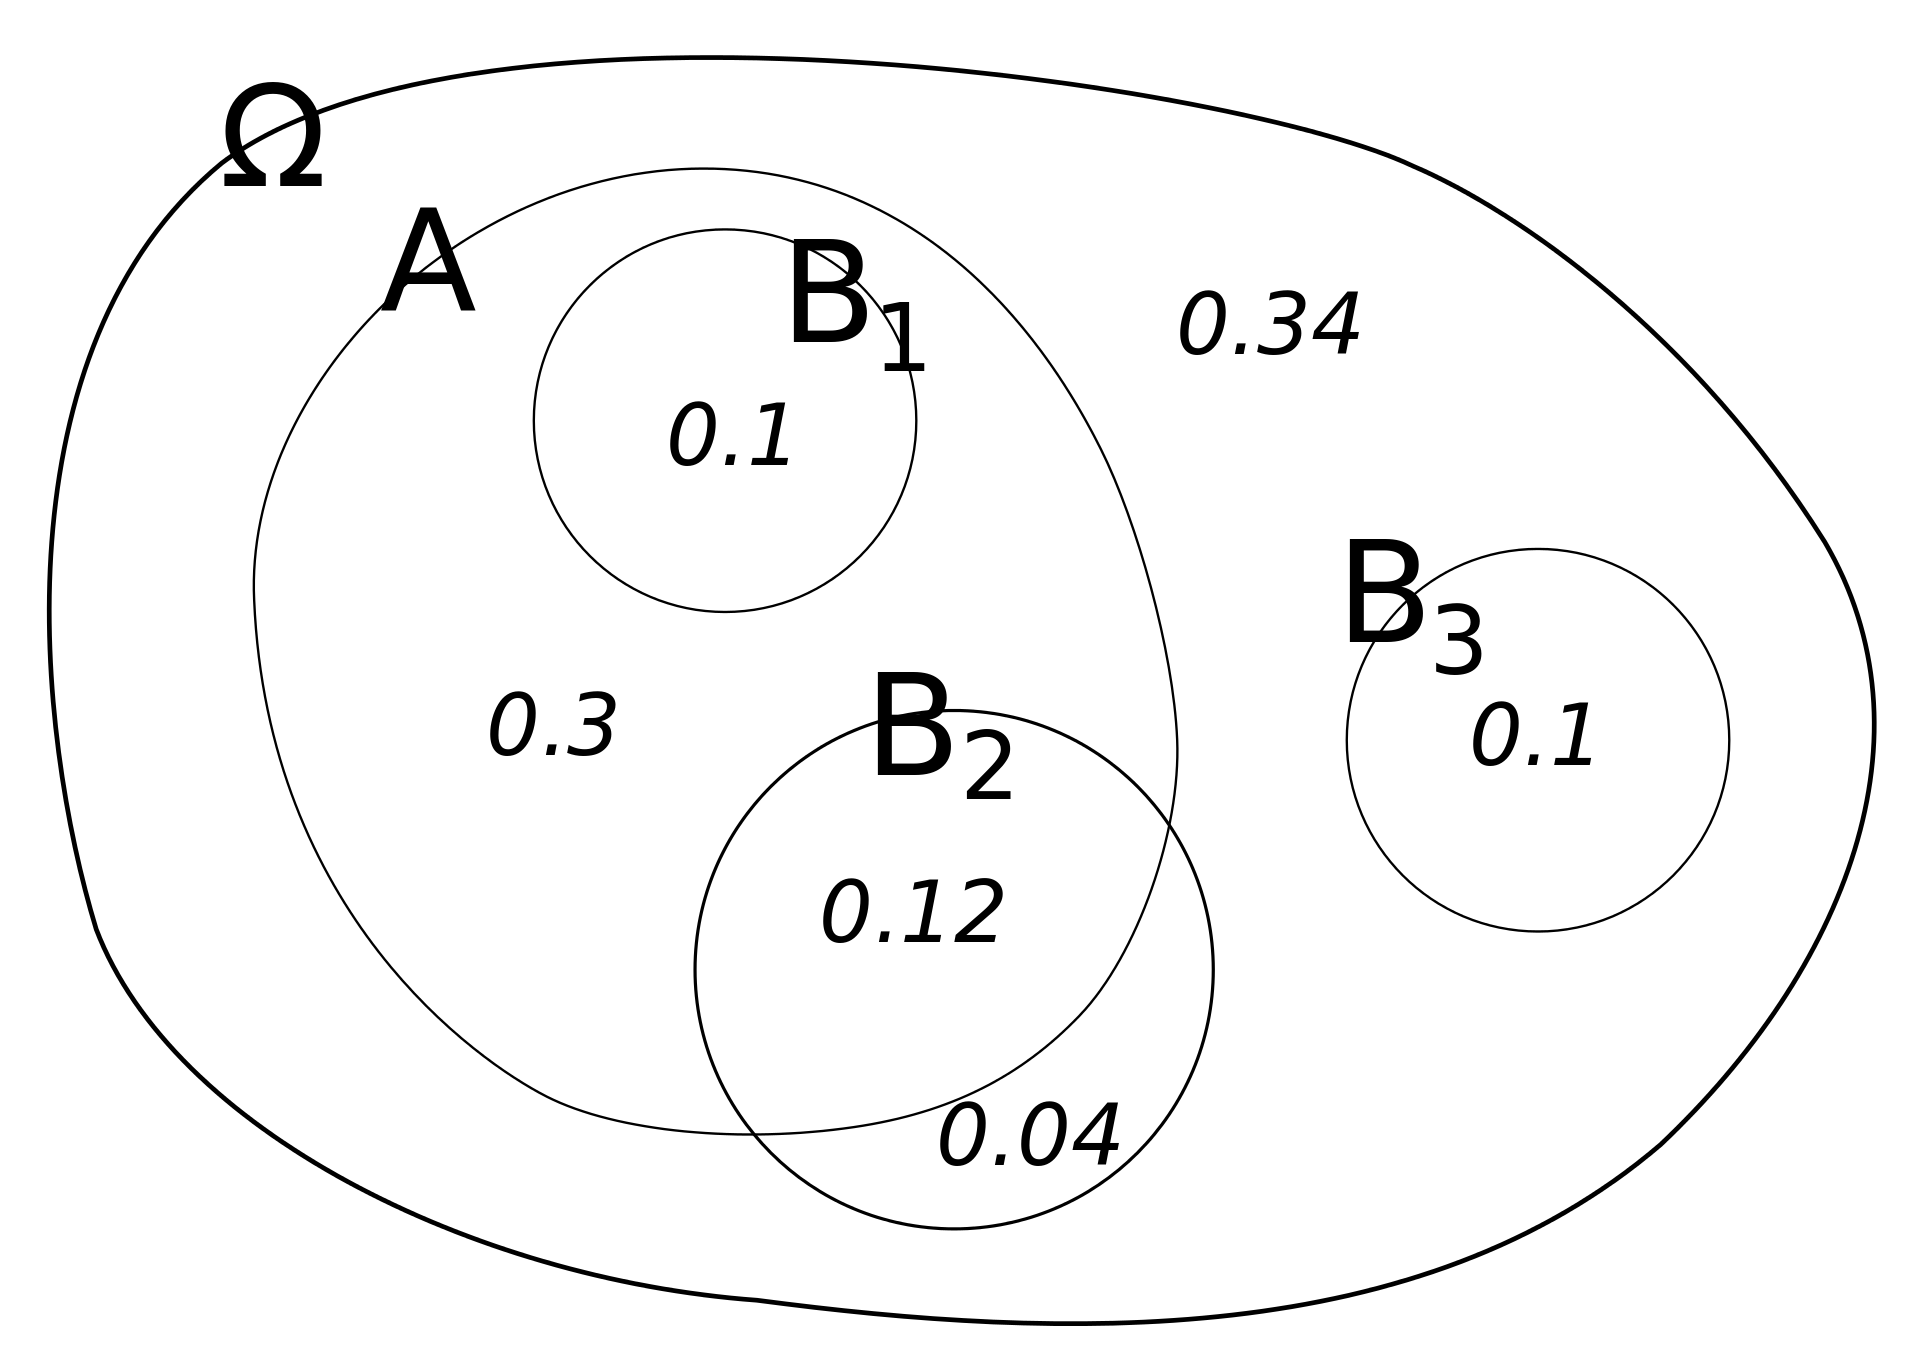
\includegraphics[width=0.4\linewidth]{Figures/Conditional_probability}
        \caption{Sets in $\Omega$ (from Wikipedia)}%
        \label{fig:conditional-prob}
    \end{figure}
    The unconditional probability $\P(A) = 0.30 + 0.10 + 0.12 = 0.52$. 
    However, the conditional probability 
    $P(A\st B_1) = 1$, 
    $P(A\st B_2) = 0.12 ÷ (0.12 + 0.04) = 0.75$, 
    and $P(A\st B_3) = 0$.
\end{example}



\begin{example}
   Here's something from Wikipedia.
   Even if 100\% of patients with pancreatic cancer have a certain symptom, when someone has the same symptom, it does not mean that this person has a 100\% 
   chance of getting pancreatic cancer. Assume the incidence rate of pancreatic cancer is 1/100000, 
   while 10/100000 healthy individuals have the same symptoms worldwide, 
   the probability of having pancreatic cancer given the symptoms is only 9.1\%, 
   and the other 90.9\% could be "false positives" (that is, falsely said to have 
   cancer; "positive" is a confusing term when, as here, the test gives bad news).
    Based on incidence rate, the following table presents the corresponding numbers per 100,000 people.
   \begin{figure}[h]
       \centering
       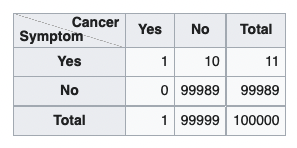
\includegraphics[width=0.4\linewidth]{Figures/cancer}
       \label{fig:cancer}
   \end{figure} 

   Which can then be used to calculate the probability of having cancer when you have the symptoms:
   \begin{align*}
&P(\text{Cancer}|\text{Symptoms})\\ &= \frac{P(\text{Symptoms}|\text{Cancer}) P(\text{Cancer})}{P(\text{Symptoms})} \\
 &= \frac{P(\text{Symptoms}|\text{Cancer}) P(\text{Cancer})}{P(\text{Symptoms}|\text{Cancer}) P(\text{Cancer}) + P(\text{Symptoms}|\text{Non-Cancer}) P(\text{Non-Cancer})} \\[8pt]
&= \frac{1 \times 0.00001}{1 \times 0.00001 + (10/99999) \times 0.99999} = \frac1{11} \approx 9.1\%
\end{align*}
\end{example}

\section{Independence}

\begin{example}
  Suppose that a fair coin is tossed twice. 
  The experiment has four outcomes, 
  $HH, HT, TH$, and $TT$, that tell us how the coin landed on each of the two tosses. 
  We can assume that this sample space is simple so that each 
  outcome has probability $1/4$. 
  Suppose that we are interested in the second toss. 
  In particular, we want to calculate the probability of the event 
  $A = \{ H \text{ on second toss}\}$. 
  We see that $A = \{HH,TH \}$, 
  so that $\P(A) = 2/4 = 1/2$. 
  If we learn that the first coin landed $T$, 
  we might wish to compute the conditional probability 
  $\P(A|B)$ where 
  $B = \{T  \text{ on first toss} \}$. 
  Using the definition of conditional probability, we easily compute  
  \begin{equation*}
      \P(A\st B) = \frac{\P(A\cap B)}{\P(B)} = \frac{1/4}{1/2} = \frac{1}{2} = \P(A) \,.
  \end{equation*}
  So, we can see that
  \begin{equation*}
      \P(A\cap B) = \P(A) \P(B) \,.
  \end{equation*}
    Another way to view this is that 
    $A$ doesn't live under the world of $B$. 
    What happens to $B$ doesn NOT affect what happens in $A$.
\end{example}

This inspires the following definition.
\begin{definition}[Independence]
   Two events $A$ and $B$ are independent if
   \begin{equation*}
       \P(A\cap B) = \P(A)\P(B)\,.
   \end{equation*}
\end{definition}

The example with the coin does not seem to have any consequence in our daily life.
However, understanding probability (or anything) could mean life or death.
There are a lot of tragedies when people misuse probability and deduce wrong conclusions
that lead to deaths of others.

\begin{example}
    In this example, we will write SIDS for Sudden Infant Death Syndrome.
    Sally Clark\footnote{\url{https://en.wikipedia.org/wiki/Sally_Clark}\\ \url{https://blogs.cornell.edu/info2040/2018/11/28/bayes-theorem-in-the-court-the-prosecutors-fallacy/}} (1964-2007) was an English woman who was wrongly accused of
    murdering her own children in 1999. 
    In the trial, certain ``expert'' Roy Meadow, calculated the following probaility:
    \begin{enumerate}
        \item $\P(\text{1 SIDS in a relatively well-off family}) \approx 1/8500$,
        \item $\P(\text{2 SIDS in a relatively well-off family}) \approx  (1/8500)^2 = 1/73 \text{million}$.
    \end{enumerate}
    From this, he concluded that this event happens once in 100 years and it is likely that Sally was guilty of killing her own children.
    The court ruled accordingly.
    This is WRONG! For a few reasons.

    \begin{enumerate}
        \item You need to look at the probability of SIDS in a typical family, not a well-off family.
            This probability turns out to be $1/1300$.
        \item Two SIDS in the same family are not two independent events.
        \item A chance for a mother to kill her own baby is \emph{incredibly low}.
    \end{enumerate}
    Let's do a conservative calculation to see the lowest chance for Sally Clark to be guilty, given the evidence provided in court.
    The key words here are ``given the evidence''.

    Let us have a few statistics up.
    Let us set up some notations.
    \begin{enumerate}
        \item $\P(\text{1 SIDS }) \approx 1/1,300$,
        \item $\P(\text{SIDS in a  family given there's already 1 SIDS}) \approx 1/130$,
        \item $\P( \text{ two children in the same household dies not from SIDS}) \approx 3/650,000$.
    \end{enumerate}

    So, from (1) and (2) already, we have
    \begin{equation*}
        \P(\text{2 SIDS in a  family}) \approx \frac{1}{1300}\frac{1}{130} = \frac{1}{169,000}\,.
    \end{equation*}
    This is still about 1/1million.
    But this still doesn't tell us about the chance that Clark murderred her children.
    Let us use the knowledge of conditional probability to proceed.
    Let $D$ denote the event of two death babies, $H$ be the event of 2 SIDS in a family, 
    Note that $H \subseteq D$. Therefore,
    \begin{align*}
        \P( H \st D) &  
        = \frac{ \P(H \cap D)  }{ \P(D)  } 
                     = \frac{ \P(H)  }{ \P(D\cap H) + \P( D \cap H^C)  } 
                     = \frac{ \P(H)  }{ \P(H) + \P(   D \st H^C) \P(H^C)   } \\
                     &\approx \frac{ 1/169,000}{ 1/169,000 + (1 - 1/169,000)* 3/650,000  } \approx 0.56\,.
    \end{align*}
    There is more chance for Sally Clark to not kill both babies than to kill. 
    This is, of course, not enough to overturn the juridiction but it is not a 
    death sentence as the previous outrageous calculation. 
\end{example}

Denote the notation
\begin{equation*}
    \sum_{i=1}^k a_i \defeq a_1 + \dots + a_k\,.
\end{equation*}

\begin{theorem}[Bayes Theorem]
    Let $(\Omega,\P)$ be a probability space.
    Let $B_1, \dots, B_k$ be disjoint events such that 
    $\P(B_i) > 0$ for $i= 1, \dots, k$ and
    \begin{equation*}
        B_1 \cup B_2 \cup \dots \cup B_k = \Omega\,.
    \end{equation*}
    Then
   \begin{equation*}
       \P(B_i\st A) = \frac{ \P(B_i\cap A) }{ \sum_{i = 1}^k \P(B_i)\P(A\st B_i)} \,.
   \end{equation*} 
\end{theorem}

\section{Random Variable and Expectation}

\begin{definition}
   Given a sample space $\Omega$. A discrete random variable $X$ is a function 
   $X:\Omega \to \N$.
\end{definition}

With this definition, we can ask what is the likelihood of $X = 1$?
Denote 
$\set{X = n}$ the event that consists of all the outcomes $\omega\in \Omega$ so that $X(\omega) = n$.

So,
\begin{equation*}
    \set{X=n} \defeq \set{ \omega \in \Omega \st X(\omega) = n}\,.
\end{equation*}
We can certainly compute 
\begin{equation*}
    \P(\set{X = n})
\end{equation*}
if we know the probability function $\P$.

\begin{definition}[Expectation]
   Let $(\Omega, \P)$ be a probability space and $X$ be a discrete random variable.
   Let $p_n = \P({X= n})$.
   The \emph{expectation} of $X$ is defined by
   \begin{equation*}
       \E(X) \defeq \sum_{n= 0}^\infty n p_n \,.
   \end{equation*}
   Sometimes we use $\mu$ to be the notation for $\E(X)$.
\end{definition}

\begin{definition}[Standard deviation]
   The \emph{variance} of $X$ is defined by 
   \begin{equation*}
      Var(X) \defeq \E( (X-\mu)^2)=   \sum_{n=0}^\infty (n - \mu)^2 p_n\,.  
   \end{equation*}
    The \emph{standard deviation} of $X$ is
    \begin{equation*}
        \sigma_X = \sqrt{Var(X)}\,.
    \end{equation*}
        
\end{definition}




